\documentclass{acm_proc_article-sp}

\begin{document}
% replace the name to unblind
\newcommand{\DataSeries}{DataSeries}
\newcommand{\DS}{DS}

\title{DataSeries: an efficient, flexible data format for structured serial data}
% Pretend we have one author, minimizes the space we waste on that.
\numberofauthors{1} 
\author{
\alignauthor
Eric Anderson, Martin Arlitt, Brad Morrey, Alistair Veitch  \\
 \affaddr{HP Labs. 1501 Page Mill Rd.  Palo Alto, CA} \\
 \email{\{eric.anderson4, martin.arlitt, brad.morrey, alistair.veitch\}@hp.com}
}

\maketitle
% % A category with the (minimum) three required fields
% \category{H.4}{Information Systems Applications}{Miscellaneous}
% %A category including the fourth, optional field follows...
% \category{D.2.8}{Software Engineering}{Metrics}[complexity measures, performance measures]
 
% \terms{Structured serial data}

% \keywords{ACM proceedings, \LaTeX, text tagging} % NOT required for Proceedings
\section{Introduction}\label{sec:intro}

DataSeries is an on-disk data format, run-time library, and set of
tools that is optimized for analyzing \textit{structured serial data},
which we define as an ordered series of records that share a common
structure.  This type of data commonly occurs as trace data in
computer systems, but since the format is essentially ordered RDBMS
tables, the need to maintain and analyze such data occurs in a large
number of scientific fields.

Traces, recordings and measurements taken from computer systems,
networks and scientific infrastructure are vitally important for a
large variety of tasks. In every area of computer system design,
traces from existing systems have been used to validate hypotheses,
test assumptions and estimate performance. This is true of I/O
subsystems~\cite{IORef,Ji03,Uysal03}, processor
systems~\cite{ProcRef}, network systems~\cite{NetRef} and memory
systems~\cite{MemRef}, among others. Traces and logs are also
extremely useful for fault-finding, auditing and debugging purposes
~\cite{DebugRef}. Traces composed of failure data have been used to
determine system reliability~\cite{ReliabilityRef, Schroeder07,
Pinheiro07}. Trend analyses of performance information is a core
operation of various management tools~\cite{MgmtRef}. Scientific and
medical instrumentation can also generate large amounts of
data~\cite{SciRef}, which also needs to be stored, filtered and
analyzed.

The data stored in each of these diverse uses is {\it structured
serial data}, which we define as a series of records, each record
having a specified structure (i.e., containing the same set of
variables). Structured serial data has four defining characteristics:
its structure is record-oriented; it is typically written only once,
not modified afterward, and is read many times; it is usually ordered
in some manner, e.g., chronologically; and it is typically read in a
sequential manner.  

There are five key properties that are desired of a data format
and analysis system for structured serial data:

\begin{enumerate}

\item \textbf{Storage efficiency}: the data should be stored in as few
bytes as possible.

\item \textbf{Access efficiency}: accessing, interpreting and encoding
trace data, whether reading or writing, should make efficient use of
CPU and memory resources.

\item \textbf{Flexibility}: adding additional fields should not affect
users of the trace data.  Removing or modifying data fields should
only affect users who use those fields and the system should support
catching incorrect usage.  Further, the format should not constrain
the type of data being stored, and should allow multiple record types
in a single file.

\item \textbf{Self-describing}: the data set should contain the
metadata that describes the data.

\item \textbf{(Re)Usability}: the data format should have an associated
programming interface that is both expressive and easy to use.

\end{enumerate}

Although numerous tracing and measurement systems have been developed
over the last 20-30 years, we are not aware of any that meet all of
these requirements. We analyze some of these in our description of
related work (section~\ref{sec:related}).

We provide four primary contributions in this paper.  First, we
introduce DataSeries, a data format and associated library, which was
specifically designed to meet the five key properties discussed above.
Second, we discuss how DataSeries can support very large datasets
(e.g., hundreds of billions of records) on modest systems.  Third, we
describe how we have used DataSeries in practice to store a wide
variety of data types.  Fourth, we demonstrate the performance and
storage efficiency of DataSeries in a set of controlled experiments,
using empirical data sets. We show that the performance of DataSeries
exceeds the performance of common trace formats and databases by at
least a factor of two, and in some cases up to an order of
magnitude. DataSeries also requires far less disk space (factors vary
from 4X to 8X in test workloads).

Since DataSeries software is publicly available (under a BSD software
license), and given the benefits of DataSeries that we demonstrate, we
argue that DataSeries should be considered for use by any application
that needs to store large amounts of structured serial data. Indeed, a
storage industry group\footnote{name withheld for blinding purposes}
has chosen DataSeries as a standard format for I/O trace data, and is
currently specifying the semantics of the fields.

The remainder of this paper is organized as follows.
Section~\ref{sec:related} describes the strengths and weaknesses of
existing storage technologies relative to DataSeries.
Section~\ref{sec:design} describes the design of DataSeries, including
on-disk and in-memory formats.
Section~\ref{sec:results} presents empirical and benchmark results
from our use of DataSeries to illustrate and quantify the benefits of
DataSeries.  Section~\ref{sec:discussion} describes our experiences
with using DataSeries, and Section~\ref{sec:conclusions} concludes the
paper with a summary of our work and a list of future directions.

\section{Related Work}\label{sec:related}

We classify the related work into three categories:
those that use a customized binary format, those that use a
text-based format, and relational database systems. 

Custom binary formats are usually serialized or directly written
versions of an in-memory data structure.  As such, they usually
achieve properties 1 and 2, and fail to achieve properties 3-5,
although as we will show in the results, unless the authors are
careful, they can also fail to achieve property 2.

Text base formats such as column separated value, or XML usually
achieve properties 3 and 4, and XML achieves property 5.  However,
they fail to achieve property 1, and can fail property two by multiple
orders of magnitude.  As we show in our results even very tuned CSV
implementations can only get to within 2-7$\times$ the
access-efficiency of DataSeries, and x-y$\times$ for the storage
efficiency.  
%{\bf TODO: need to re-do these experiments at least to
%measure the file sizes, and potentially with Tfrac text files,
%although I suspect people would use sec.usec in a block I/O trace}

Relational databases achieve properties 3, 4, and 5. RDBMS's were
designed to handle updates, so do very limited compression drastically
hurting their storage efficiency (property 1).  Our results show
$>$10x improvement on storage efficiency for DataSeries over
MySQL. 
%{\bf TODO: check the exact sizes, should be around there.}
Similarly, the generality of SQL can hurt it.  Even for fairly simple
queries running entirely in the database, DataSeries runs 2-7$\times$
faster than MySQL. 
%{\bf TODO: re-do these numbers with parallel
%decompression, etc.}  
Retrieving the data for a more complicated
calculation on the client would further slow the relative performance.

\section{Design}\label{sec:design}

DataSeries' data model is conceptually very similar to that used by
relational databases.  Logically, a DataSeries file is composed of an
ordered sequence of {\it records}, where each record is composed from
a set of {\it fields}. Each field has a {\it field-type} (e.g.,
integer, string, double, boolean) and a name. A DataSeries record is
analogous to a row in a conventional relational database. We call the
type of a row the {\it extent-type} because an {\it extent} contains a
collection of rows with the same fields and field-types.

A single DataSeries file comprises a collection of extents
(potentially with different extent-types), plus a header and
extent-type extent at the beginning of the file, and an index extent
and trailer at the end of the file. Figure~\ref{fig:dsorg} shows this
organization.  The header on a DataSeries file contains the DataSeries
file version, and endianness encodings of the data types.  The
extent-type extent contains records with a single string-valued field,
each of which contains an XML specification that defines the
extent-types of all the other extents in the file. The trailer
consists of the offset and size (after compression) of the index
extent.  The offset is used to read the index extent, which has two
fields, an extent-type and an offset, to allow direct access to
extents of a single type.

\begin{figure*}
% \vspace{-0.6cm}
\hfil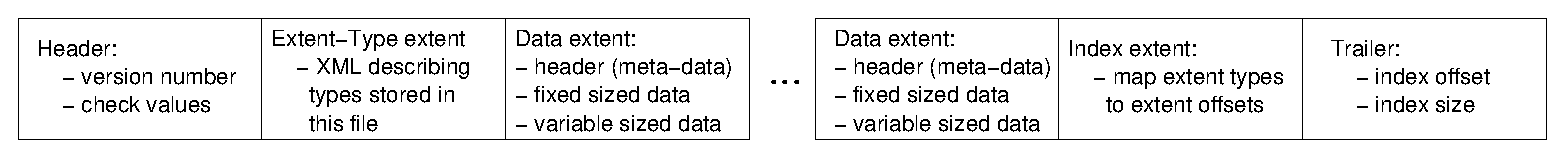
\includegraphics[width=6.5in]{tr-fig/ds-format2.eps}\hfil
\caption{Internal structure of a DataSeries file. }
\label{fig:dsorg}
% \vspace{-2mm}
\end{figure*}

The data extents themselves consist of a header, followed by the fixed
size data and the variable sized data.  Both fixed and variable sized
data may be compressed, using any one of a number of standard
compression algorithms~\cite{GZIP,BZIP,LZF,LZO}.  The header contains
metadata about the data in the extent, such as the compressed sizes of
the fixed and variable data, the number of records in the extent, the
uncompressed size of the variable length data, the compression mode,
the extent-type of the extent, and checksums of the extent before and
after compression to guard against hardware and software errors.
Checksum validation can be disabled during extent reading to improve
performance at the cost of reduced reliability.

DataSeries supports a number of options that control either the
interpretation of a field (e.g. can it be null), or the way the field
is represented prior to compression ({\em packed}, e.g. relative to
another field).  DataSeries also has some options for representation
of entire extents (e.g. ordering of the fields in a record).  The
packing options are handled transparently by DataSeries, the
interpretation options are checked against the field accessors.
Detailed explanation of the options can be found in the DataSeries
technical report~\cite{DSTechnicalReportSnapshot}.

Programming is in the TR.  There are also lots of modules to help; see
the TR.  Mention dstypes2cxx here also.

\section{Performance Results}\label{sec:results}

We performed various experiments to measure the effectiveness of
\DataSeries{}' compression techniques, and then further compared \DataSeries{} to data encoding and analysis using MySQL, CSV, CStore, Dan Ellard's Harvard traces\cite{ellard03}, and the 1998 World Cup Web traces\cite{ita08} for compression ratio and analysis execution speed.  Due to space constraints we simply give example results
from our comparison with Ellard and the World Cup.  More complete coverage can be found in the DataSeries technical report~\cite{DSTechnicalReportSnapshot}.


\subsection{Ellard Traces}\label{sec:ellard}

In an effort to experiment with using DataSeries to represent and
analyze traces generated by other people, we converted Daniel Ellard's
Harvard traces\cite{ellard03} into DataSeries.  The Ellard traces
were originally stored as compressed text files, one record per line.
The first part of each line is a series of fixed fields, followed by a
set of key-value pairs, and finally some debugging information.  As
part of the tools, there is also a scanning program which reads the
trace files and outputs summary information for a trace.

Our evaluation came in two parts.  First, we wrote programs that
converted between the two formats.  The reversable conversion
guaranteed that we were properly preserving all of the information.
We found that the DataSeries files were on average 0.74x the size of
the original files when both were compressed using gzip.  Second, we
wrote an analysis program that implemented the first three examples in
the README that came with the tools.  We found that our analysis
program ran about 76x faster on those data files than the text
analysis program that came with the distribution.  
We also found that if we utilized lzo compression, which decompresses
more quickly than gzip,
our analysis program
ran about 107x faster, in exchange for slightly larger (1.14x) data files.

% Move this so it shows up on same page as reference.
\begin{table*}[t]
\centering
\begin{tabular}{|c|c|c|c|c|c|c|}\hline
Trace Set & gz-64k  & gz-128k & gz-512k & lzo-64k & lzo-128k & bzip2-16M \\ \hline
overall   & 0.9459x & 0.8531x & 0.7721x & 1.1387x & 1.0437x & 0.76x   \\
deasna    & 0.9800x & 0.8856x & 0.7996x & 1.1535x & 1.0552x & 0.8064x \\
deasna2   & 1.0003x & 0.8976x & 0.8051x & 1.1680x & 1.0614x & 0.8148x \\
home02    & 0.9111x & 0.8204x & 0.7440x & 1.1252x & 1.0335x & 0.7084x \\
home03    & 0.9059x & 0.8170x & 0.7422x & 1.1197x & 1.0301x & 0.7073x \\
home04    & 0.8974x & 0.8094x & 0.7358x & 1.1148x & 1.0261x & 0.6979x \\
lair62    & 0.9663x & 0.8949x & 0.8271x & 1.1153x & 1.0427x & 0.8145x \\
lair62b   & 0.9859x & 0.8883x & 0.8009x & 1.1597x & 1.0579x & 0.8438x \\
\hline
\end{tabular}

\caption{Compression ratios for the different options.  The gz and lzo
columns are compared relative to the gzip compressed text files.  The
bzip2 results are compared to bzip2 compressed text files.  The
results exclude the 8 files with zero blocks in them.  The sizes after
the compression ratio is the extent size used for the DataSeries files.}

\label{table:ellard:compression}
\end{table*}

\subsubsection{Compression comparison}

Table~\ref{table:ellard:compression} shows the DataSeries compression results
relative to the original Ellard traces.  The compression difference
using bzip2 compression is slightly lower than with gzip, the
DataSeries files are 0.76x smaller than the text files compressed
using bzip2.  We compared the lzo files to the gzip compressed files
since for the text files compression with lzo would offer no benefit,
the files would be larger and the wall time for analysis would be the
same.  For gzip we tested with extent sizes of 64k, 128k and 512k.
For lzo, we tested with extent sizes of 64k and 128k.

We have not investigated what causes the difference in the compressed
file sizes.  We have observed that for the small extent sizes
(64k/128k) the compressed extents are very small (5-10k), which means
that some of the DataSeries per-extent overhead may be contributing to
the larger size, as well as the compression algorithms may not have
enough data to fill their window.

\subsubsection{Performance comparison}

For the performance comparison, we implemented a subset of the
analysis performed by Ellard's \texttt{nfsscan} program. In particular one
that can perform the first three of the five example questions
presented in the EXAMPLES file that comes with Ellard's trace tools.
This analysis turned out to be very simple, it is just counting the
number of requests performed of each client of each type.  We chose to
implement this over the integer operation id, rather than the string,
and so wrote a short table that converted NFSv2 and NFSv3 operation
id's into a common space. The performance comparison was done using
DataSeries revision 61f07e212acb972da6c603bed82ab2ec5ca1b731 from
2008-01-21.

All of our experiments were performed on a DL365g1 with 8 GB memory,
2x 2.4GHz dual-core Opteron 2216 HE.  Data was stored on nfs.
Ellard's \texttt{nfsscan} program was run \texttt{zcat (or bzcat) $|$
nfsscan -t0 -BC -}, so we get separate times for the decompression and
nfsscan execution, but a single elapsed time.  The detailed
measurements can be found in the DataSeries distribution in
\texttt{doc/tr/ellard-details.tex}.

\begin{table*}
\centering
\begin{tabular}{|c|c|c|c|c|c|c|} \hline
            & mean     & mean       & mean     & CPU     & mean     & Wall time \\
algorithm   & user (s) & system (s) & CPU (s)  & speedup & wall (s) & speedup  \\ \hline
ellard-gz   & 537.58    &  7.80     & 545.38   &  1.0x   & 545.71   &   1.0x   \\
ellard-bz2  & 638.48    & 12.68     & 651.16   &  0.836x & 571.49   &   0.955x \\
\hline
ds-gz-512k  &  22.91    &  3.62     &  26.53   & 20.557x &   7.16   &  76.186x \\
ds-gz-64k   &  21.45    &  1.14     &  22.59   & 24.147x &   5.81   &  93.945x \\
ds-gz-128k  &  23.30    &  1.19     &  24.49   & 22.268x &   6.30   &  86.604x \\
\hline
ds-bz2-16M  &  94.38    & 11.82     & 106.20   &  5.136x &  27.66   &  19.732x \\
ds-lzo-64k  &  18.71    &  1.14     &  19.85   & 27.472x &   5.10   & 106.897x \\
ds-lzo-128k &  21.15    &  1.10     &  22.25   & 24.514x &   5.74   &  95.022x \\
ds-lzo-512k &  24.07    &  4.07     &  28.14   & 19.382x &   7.40   &  73.762x \\ \hline
\end{tabular}

\caption{Summary of performance results for the two analysis programs
operating on a variety of input files.  The analysis was run over the
anon-home04-011118-* files.  For the ellard \texttt{nfsscan} program
the text files were compressed with either gz or bz2.  For the
DataSeries \texttt{ellardanalysis} program, the dataseries files were
compressed with either gz, bz2, or lzo, and used various extent sizes
as specified.  CPU and wall time are both relative to ellard-gz.}

\label{tab:summary}
\end{table*}


Table~\ref{tab:summary} presents the summary results, showing the
impressive speedup and reduction in CPU time that can be achieved by
using DataSeries.  The different sizes specified after the compression
algorithm for the DataSeries rows are the extent sizes. 
The substantial increase in system time for dealing
with large extents for bzip2 is a result of glibc's use of mmap/munmap
for large allocations.  Every extent results in a separate pair of
mmap/munmap calls to the kernel and hence a substantial about of page
zeroing in the kernel.  The detailed measurements can be found 
in the DataSeries distribution in \texttt{doc/tr/ellard-details.tex}.

\subsection{1998 World cup traces}\label{sec:world-cup-1998}

The 1998 World cup traces\cite{ita08} are one of the largest
publically available web traces.  They were collected from the many
web servers for the 1998 World Cup games.  We converted the traces
from the special raw format used for them into DataSeries, and also
created a version of the {\tt checklog} program that comes with the
traces as a comparison point for analysis.  For these traces, we found
that conversion to DataSeries files were on average 0.93$\times$ the
size of the original files, and that the analysis program used about
YY$\times$ less CPU time and ran about ZZ$\times$ faster.
% YY = 1.5, ZZ = 2 on my laptop

\subsubsection{Conversion to and from DataSeries}

Table~\ref{table:wc1998:compression} shows the overall compression of
the different options.  The \{le,be\}-\{bts,stb\}-gz files are the
original data files stored in little or big endian format (le/be) and
big to small or small to big (bts/stb) ordering.  The original traces
are be-bts-gz.  The DataSeries file without any options is ds-base,
and then options can be added on for reducing the field padding to the
maximum column size (mcs), packing the fields in big to small order
(bts), or packing the time field self-relative (tsr).

% plots and tables can be re-generated using graphs/wc1998/plot.hg

\begin{table}
\centering
\begin{tabular}{|c|c|c|c|}\hline

               &            & ratio to & ratio to \\
    dataset    & size (MiB) & ds-base & be-bts-gz \\
\hline							   
ds-mcs-bts-tsr & 7648.98  & 1.133         & 1.077         \\
ds-mcs-tsr     & 7722.78  & 1.122         & 1.067         \\
ds-bts-tsr     & 7890.12  & 1.098         & 1.044         \\
ds-tsr         & 8065.99  & 1.074         & 1.021         \\
le-bts-gz      & 8152.47  & 1.063         & 1.011         \\
ds-mcs-bts     & 8183.98  & 1.059         & 1.007         \\
be-bts-gz      & 8239.15  & 1.052         & 1.000         \\
le-stb-gz      & 8391.09  & 1.032         & 0.982         \\
be-stb-gz      & 8411.46  & 1.030         & 0.980         \\
ds-mcs         & 8423.56  & 1.029         & 0.978         \\
ds-bts         & 8439.72  & 1.027         & 0.976         \\
ds-base        & 8663.78  & 1.000         & 0.951         \\
\hline
\end{tabular}


\caption{Compression options for the data files sorted from the smallest 
to the largest.  Gzipped files can be stored little or big endian
(le/be) and small to big or big to small (stb/bts).  DataSeries files
can be stored with the fields padded only to the maximum column size
(mcs), with the fields stored big to small (bts), or with the time
field packed self relative (tsr). be-bts-gz is the original 1998 World
Cup trace format.}

\label{table:wc1998:compression}
\end{table}

\subsubsection{Analysis performance}

We re-implemented the {\tt checklog} program that comes with the 1998
World Cup traces.  That program calculates a couple of the values in
multiple ways.  We duplicated this calculation because we wanted the
programs to be comparable, even though performing the calculation is
unnecesary. When running the program we found that the DataSeries
implementation ran ZZ$\times$ faster.  This result was expected as the
analysis performed was fairly simple, and as DataSeries used multiple
CPUs for decompression, it was able to run faster.  However, we also
found that the implementation used about YY$\times$ less CPU.  This
was unexpected given that DataSeries was using a virtual function call
for every row, and was having to process the extents separately.  We
examined the CPU utilization using oprofile and valgrind and found
that the original code had three problems:

\begin{itemize}

\item {\bf Non-integrated decompression}.  The {\tt checklog} program 
used a separate process to perform the decompression, this led to
slightly increased system time to pass the data over the pipe.

\item {\bf Very slow byte-swapping routine}.  The {\tt checklog} program
had to byte-swap every record, and the implementation used for
byte-swapping was very slow.  Moreover, the implementation copied the
data rather than doing the byte-swapping in-place, further increasing
the overhead.

\item {\bf Slow per-record fread}.  The {\tt checklog} program called 
fread for each record.  While we didn't expect this to be slow, it
turned out that the implementation is slow, and so calling fread for
each record is a poor choice.

\end{itemize}

While we could re-implement {\tt checklog}, it doesn't seem
particularly valuable.  The expected end result would be that the
checklog program would use less CPU time than the DataSeries program,
but would use more wall-clock time because there is no easy way to
parallelize the reading of the underlying files.



\section{Practical Experiences}\label{sec:discussion}

The largest dataset we have is NFS data we have collected.  The primary extent type 
in this data is the common records which store information about each
of the 200 billion request and reply messages. We have secondary tables that
store information about each packet captured, operations that included
file attributes, read and write requests and mount requests.  The total dataset
is about 5TB in size.

As a demonstration of the real-life performance of
\DataSeries{}, consider the following example.  Utilizing a trace of NFS
traffic from a LAN, we performed an analysis of the throughput
effects if servers were instead accessed across a WAN.
The analysis read in 45.5 GB of data (406 GB when uncompressed), and
processed 7.6 billion records (each record corresponds to an NFS
transaction).  Using a four year old two-way 2.8 GHz Xeon server, the
entire data set was processed in 11,263 wall clock seconds (about 3
hours), or roughly 675,000 rows per second performing a set of complex
analyses.

As a second demonstration of real life performance we used
\DataSeries{} to build a large set of reports and graphs from LSF
data.  Some of our reports were similar to ones already being created
through queries to a commercial relational database.  Report
generation in \DataSeries{} ran over 50$\times$ faster than the
database report generation.  While we did not investigate precisely
why the database version was slower, it appeared to come from two
sources.  First, \DataSeries{} is entirely targeted at analysis, and
hence runs those calculations very efficiently.  Second, the desired
calculations would require many SQL queries to generate the same
results as the single pass \DataSeries{} calculation, and it is likely
the queries were executed sequentially for simplicity in the program
generating the report.



\section{Conclusions}\label{sec:conclusions}

We have described \DataSeries{}, a data format that enables the efficient
and flexible storage of structured serial data. This type of data is
used in numerous applications in all areas of computing
and science, and researchers have developed almost as many ways to
store and process it as there are applications. Unfortunately, there are
many limitations to these formats. In contrast, \DataSeries{} offers five major
advantages:
\begin{enumerate}
\item \DataSeries{} improves \textit{storage efficiency}, by
 incorporating compression algorithms and related techniques.  Using
 \DataSeries{}, we have been able to store and analyze large datasets on
 a significantly smaller server and storage system than is typically
 used with databases.

\item \DataSeries{} provides much better \textit{access efficiency} than
other formats.  This enables the timely analysis of very large datasets.

\item \DataSeries{} is \textit{flexible}, in that it can handle a wide variety of
different types of data, multiple types of data in the same file, and
is easily extensible to handle new data types without changing the
format. In fact, in almost four years of use, and an increasing number of
data types, including I/O traces (disk block and NFS), batch cluster logs, 
system call traces, performance measurements and email content, we have 
not had to update the format once.

\item \DataSeries{} is \textit{self-describing}; that is, relevant metadata is retained with the data.

\item \DataSeries{} has an API to improve the \textit{usability} of the format by others.
\end{enumerate}

DataSeries is open source that can be downloaded from {\tt
http://tesla.hpl.hp.com/opensource/}

\bibliographystyle{abbrv}
{\small
\bibliography{tr-references}
}
% You must have a proper ".bib" file
%  and remember to run:
% latex bibtex latex latex
% to resolve all references
%
% ACM needs 'a single self-contained file'!
%
\balancecolumns

\end{document}
